%Dokumentinformationen
\newcommand{\titleinfo}{Analysis 2E - Formelsammlung}
\newcommand{\authorinfo}{F. Braun, L. Schmid, U. Giger, R. Koller, E. Ammann, S.
Arnold}
\newcommand{\versioninfo}{$Revision: 813 $ - powered by \LaTeX}

% standard header

%Dokumentinformationen
\newcommand{\titleinfo}{Analysis 2E - Formelsammlung}
\newcommand{\authorinfo}{KKK K\"oppel, K\"oppel und Konsortium, basierend auf
Sammlung von F. Braun \& Co}
\newcommand{\versioninfo}{$Revision: 2.0 $}



%%%%%%%%%%%%%%%%%%%%%%%%%%%%%%%%%%%%%%%%%%%%%%%%%%%%%%%%%%%%%%%%%%%%%%%%%%%%%%%%%%%%%%%%%%%%%%%%
% Neue Befehle und Definitionen                
%%%%%%%%%%%%%%%%%%%%%%%%%%%%%%%%%%%%%%%%%%%%%%%%%%%%%%%%%%%%%%%%%%%%%%%%%%%%%%%%%%%%%%%%%%%%%%%

\newcommand{\formelbuch}[1]{$_{\textcolor{red}{\mbox{\small{S#1}}}}$}
\newcommand{\verweis}[2]{\small{(siehe auch \ref{#1}, #2 (S. \pageref{#1}))}}
\newcommand{\subsubadd}[1]{\textcolor{black}{\mbox{#1}}}




%Schriftgr�sse, Layout, Papierformat, Art des Dokumentes
\documentclass[10pt,twoside,a4paper,fleqn]{article}
%Einstellungen der Seitenr�nder
\usepackage[left=1cm,right=1cm,top=1cm,bottom=1cm,includeheadfoot]{geometry}
% Sprache, Zeichensatz, packages
\usepackage[latin1]{inputenc}
\usepackage[ngerman]{babel,varioref}
\usepackage{amssymb,amsmath,fancybox,graphicx,color,lastpage,wrapfig,fancyhdr,hyperref,verbatim}

%Teile des Dokuments Mehrspaltig
\usepackage{multicol}
%Rotieren von Elementen (Bilder, Tabellen...)
\usepackage{rotating}

%Fliesstext
\usepackage{wrapfig}

%pdf info
\hypersetup{pdfauthor={\authorinfo},pdftitle={\titleinfo},colorlinks=false}
%linkbordercolor=white
\author{\authorinfo}
\title{\titleinfo}

%Kopf- und Fusszeile
\pagestyle{fancy}
\fancyhf{}
%Linien oben und unten
\renewcommand{\headrulewidth}{0.5pt} 
\renewcommand{\footrulewidth}{0.5pt}

\fancyhead[L]{\titleinfo{ }\tiny{(\versioninfo)}}
%Kopfzeile rechts bzw. aussen
\fancyhead[R]{Seite \thepage { }von \pageref{LastPage}}
%Fusszeile links bzw. innen
\fancyfoot[L]{\footnotesize{\authorinfo}}
%Fusszeile rechts bzw. ausen
\fancyfoot[R]{\footnotesize{\today}}

\definecolor{black}{rgb}{0,0,0}
\definecolor{red}{rgb}{1,0,0}
\definecolor{white}{rgb}{1,1,1}
\definecolor{grey}{rgb}{0.8,0.8,0.8} % ./header.tex nicht editieren (Projekt LaTeX-Header benutzen)

%%%%%%%%%%%%%%%%%%%%%%%%%%%%%%%%%%%%%%%%%%%%%%%%%%%%%%%%%%%%%%%%%%%%%%%%%%%%%%%%%%%%%%%%%%%%%%%%
% Neue Befehle und Definitionen                
%%%%%%%%%%%%%%%%%%%%%%%%%%%%%%%%%%%%%%%%%%%%%%%%%%%%%%%%%%%%%%%%%%%%%%%%%%%%%%%%%%%%%%%%%%%%%%%
\definecolor{black}{rgb}{0,0,0}
\definecolor{red}{rgb}{1,0,0}
\definecolor{white}{rgb}{1,1,1}
\definecolor{grey}{rgb}{0.8,0.8,0.8}
\newcommand{\formelbuch}[1]{$_{\textcolor{red}{\mbox{\small{S#1}}}}$}
\newcommand{\verweis}[2]{\small{(siehe auch \ref{#1}, #2 (S. \pageref{#1}))}}
\newcommand{\subsubadd}[1]{\textcolor{black}{\mbox{#1}}}

\begin{document}

\setlength{\parindent}{0pt}

\section{Integralrechnung \formelbuch{483}}
\subsection{Integrationsmethoden \formelbuch{486ff}}
  
  \begin{tabular}{ll}
    Linearit\"at & $\int{f(\alpha x+\beta )dx=\frac{1}{\alpha}\cdot F(\alpha x+\beta)+C}$ \\
    Partielle Integration & $\int\limits_a^b{u'(x)\cdot v(x)dx}=\biggl[
    u(x)\cdot v(x) \biggr]_a^b-\int\limits_a^b{u(x)\cdot v'(x)dx}$\\
    Substitution (Rationalisierung) & $t=\tan\frac{x}{2}, \qquad
    dx=\frac{2dt}{1+t^2} \qquad \sin  x=\frac{2t}{1+t^2} \qquad \cos x=\frac{1-t^2}{1+t^2}
    \quad\int{R(\sin(x)\cos(x))dx}$\\
    Allgemeine Substitution &
    $\int\limits_{a}^{b}{f(x)dx}=\int\limits_{g^{-1}(a)}^{g^{-1}(b)}{f(g(t))\cdot
    g'(t)dt}\qquad t=g^{-1}(x)\qquad  \fbox{x=g(t)}\qquad dx=g'(t)\cdot dt$\\
    Logarithmische Integration & $\int{\frac{f'(x)}{f(x)}dx}=\ln|f(x)|+C 
    \qquad{(f(x)\neq 1)}$\\
    Spezielle Form des Integranden & $\int{f'(x)\cdot (f(x))^{\alpha} dx}=
    f(x)^{\alpha +1}\cdot \frac{1}{\alpha+1}+C
    \qquad{(\alpha \neq -1)}$\\
    Differentiation & $\int \limits ^{b} _{a} {f'(t)dt}=f(b)-f(a)$\\
    & $\frac{d}{dx} \int \limits ^{x} _{1} {f(t)dt}=f(x)$
  \end{tabular}
  
  

\subsubsection{Einige unbestimmte Integrale \formelbuch{1074 ff}}
  \begin{enumerate}
    \item $ \int dx=x+C $
    \item $ \int{x^\alpha}dx=\frac{x^{\alpha+1}}{\alpha+1}+C,\ x \epsilon \mathbb
    R ^+,\ \alpha \epsilon \mathbb R \backslash \{ -1 \} $
    \item $ \int{\frac{1}{x}}dx=\ln \left| x \right| + C,\ x\neq0 $
    \item $ \int{e^x}dx=e^x+C $
    \item $ \int{a^x}dx=\frac{a^x}{\ln{a}}+C,\ a \epsilon \mathbb
    R^+\backslash\{1\} $
    \item $ \int{ \sin{x}} dx = -\cos{x} + C $
    \item $ \int{\cos{x}} dx = \sin{x} + C $
    \item $ \int{\frac{dx}{\sin^2x}}=-\cot{x}+C,\ x\neq k\pi\ \mathrm{mit}\ k
    \epsilon \mathbb Z $
    \item $ \int{\frac{dx}{\cos^2x}}=\tan{x}+C,\ x\neq\frac{\pi}{2}+k\pi\
    \mathrm{mit} k \epsilon \mathbb Z $
    %10. :
    \item $ \int{\sinh{x}}dx = \cosh{x}+C $
    \item $ \int{\cosh{x}}dx = \sinh{x}+C $
    \item $ \int{\frac{dx}{\sinh^2x}}=-\coth{x}+C,\ x\neq0 $
    \item $ \int{\frac{dx}{\cosh^2x}}=\tanh{x}+C $
    \item $ \int{\frac{dx}{ax+b}} = \frac{1}{a}\ln \left|ax + b\right| + C,\
    a\neq 0,x\neq-\frac{b}{a} $
    \item $ \int{\frac{dx}{a^2x^2+b^2}}=\frac{1}{ab}\arctan{\frac{a}{b}x}+C,\
    a\neq0,\ b\neq0 $
    \item $
    \int{\frac{dx}{a^2x^2-b^2}}=\frac{1}{2ab}\ln{\left|\frac{ax-b}{ax+b}\right|}+C,\ a\neq0,\ b\neq0,\ x\neq\frac{b}{a},\ x\neq-\frac{b}{a} $
    \item $
    \int{\sqrt{a^2x^2+b^2}}dx=\frac{x}{2}\sqrt{a^2x^2+b^2}+\frac{b^2}{2a}\ln{(ax+\sqrt{a^2x^2+b^2})}+C,\
    a\neq0,\ b\neq0 $
    \item $
    \int{\sqrt{a^2x^2-b^2}}dx=\frac{x}{2}\sqrt{a^2x^2-b^2}-\frac{b^2}{2a}\ln\left|ax+\sqrt{a^2x^2-b^2}\right|+C,\
    a\neq0,\ b\neq0,a^2x^2\geqq b^2$
    \item $
    \int\sqrt{b^2-a^2x^2}dx=\frac{x}{2}\sqrt{b^2-a^2x^2}+\frac{b^2}{2a}\arcsin\frac{a}{b}x+C,\
    a\neq0,\ b\neq0,\ a^2x^2\leqq b^2 $
    %20.:
    \item $
    \int\frac{dx}{\sqrt{a^2x^2-b^2}}=\frac{1}{a}\ln(ax+\sqrt{a^2x^2+b^2})+C,\
    a\neq0,\ b\neq0 $
    \item $
    \int\frac{dx}{\sqrt{a^2x^2-b^2}}=\frac{1}{a}\ln\left|ax+\sqrt{a^2x^2-b^2}\right|+C,\
    a\neq0,\ b\neq0,\ a^2x^2>b^2 $
    \item $ \int\frac{dx}{\sqrt{b^2-a^2x^2}}=\frac{1}{a}\arcsin\frac{a}{b}x+C,\
    a\neq0,\ b\neq0,\ a^2x^2<b^2 $
    \item Die Integrale $\int\frac{dx}{X}, \int\sqrt{X}dx,
    \int\frac{dx}{\sqrt{X}}$ mit $X=ax^2+2bx+c,\ a\neq0 $ werden durch die
    Umformung $X=a(x+\frac{b}{a})^2+(c-\frac{b^2}{a}) $ und die Substitution $
    t=x+\frac{b}{a} $ in die Integrale 15. bis 22. transformiert.
    \item $
    \int\frac{xdx}{X}=\frac{1}{2a}\ln\left|X\right|-\frac{b}{a}\int\frac{dx}{X},\ a\neq0,\ X=ax^2+2bx+c$
    \item $ \int\sin^2axdx=\frac{x}{2}-\frac{1}{4a}\cdot\sin2ax+C,\ a\neq0 $
    \item $ \int\cos^2axdx=\frac{x}{2}+\frac{1}{4a}\cdot\sin2ax+C,\ a\neq0 $
    \item $ \int\sin^naxdx=-\frac{sin^{n-1}ax\cdot\cos
    ax}{na}+\frac{n-1}{n}\int\sin^{n-2}axdx,\ n \epsilon \mathbb N,\ a\neq0 $
    \item $ \int\cos^naxdx=\frac{\cos^{n-1}ax\cdot\sin
    ax}{na}+\frac{n-1}{n}\int\cos^{n-2}axdx,\ n\epsilon \mathbb N,\ a\neq0 $
    \item $ \int\frac{dx}{\sin ax} =
    \frac{1}{a}\ln\left|\tan\frac{ax}{2}\right|+C,\ a\neq0,\ x\neq
    k\frac{\pi}{a}\ \mathrm{mit}\ k\epsilon\mathbb Z$
    %30.:
    \item $ \int\frac{dx}{\cos
    ax}=\frac{1}{a}\ln\left|\tan(\frac{ax}{2}+\frac{\pi}{4})\right|+C,\ a\neq0,\
    x\neq\frac{\pi}{2a}+k\frac{\pi}{a}\ \mathrm{mit}\ k\epsilon\mathbb Z $
    \item $\int\tan axdx=-\frac{1}{a}\ln\left|\cos ax\right|+C,\ a\neq0,\
    x\neq\frac{\pi}{2a}+k\frac{\pi}{a} \mathrm{mit}\ k\epsilon\mathbb Z$
    \item $\int\cot axdx=\frac{1}{a}\ln\left|\sin ax\right|+C,\ a\neq0,\ x\neq
    k\frac{\pi}{a} \mathrm{mit} k\epsilon\mathbb Z $
    \item $ \int x^n\sin axdx=-\frac{x^n}{a}\cos ax+\frac{n}{a}\int x^{n-1}\cos
    axdx,\ n\epsilon\mathbb N,\ a\neq0 $
    \item $ \int x^n\cos axdx=\frac{x^n}{a}\sin ax-\frac{n}{a}\int x^{n-1}\sin axdx,\ n\epsilon\mathbb N,\ a\neq0 $
    \item $ \int x^ne^{ax}dx=\frac{1}{a}x^ne^{ax}-\frac{n}{a}\int
    x^{n-1}e^{ax}dx,\ n\epsilon\mathbb N,\ a\neq0 $
    \item $ \int e^{ax}\sin bxdx=\frac{e^{ax}}{a^2+b^2}(a\sin bx-b\cos bx)+C,\
    a\neq0,\ b\neq0 $
    \item $ \int e^{ax}\cos bxdx=\frac{e^{ax}}{a^2+b^2}(a\cos bx + b\sin bx)+C,\
    a\neq0,\ b\neq0 $
    \item $ \int\ln x dx = x(\ln x-1)+C,\ x\epsilon\mathbb R^+ $
    \item $ \int x^\alpha \cdot \ln xdx =
    \frac{x^{\alpha+1}}{(\alpha+1)^2}\lbrack(\alpha+1)\ln x-1\rbrack + C,\
    x\epsilon\mathbb R^+,\ \alpha\epsilon\mathbb R\backslash\{-1\} $
    %FF1 Seite 496
  \end{enumerate}

  Uneigentliches Integral heisst, dass entweder eine \textbf{unbeschr\"ankte
  Funktion} integriert wird, oder eine Funktion \"uber einen
  \textbf{unbeschr\"ankten Integrationsberech} integriert wird.\\


  \begin{multicols}{2}
    F\"ur unbeschr\"ankte Funktionen:\\
    $ I =\int\limits _{a}^{c}f(x)dx=\lim\limits_{t\to
    b-}\int\limits_{a}^{t}f(x)dx+\lim\limits_{t\to b+}\int\limits_{t}^{c}f(x)dx
    $ \\
    F\"ur die unbeschr\"ankte Integration:\\
    $ I =\int\limits _{a} ^{\infty} f(x)dx= \lim \limits_{t\to \infty}\int \limits
    _{a} ^{t}f(x)dx; $ \\
    $ I =\int\limits ^{a} _{-\infty} f(x)dx= \lim \limits_{t\to -\infty}\int
    \limits _{t} ^{a}f(x)dx; $ \\
    $I =\int\limits _{-\infty} ^{\infty} f(x)dx = \lim \limits_{t_1\to \infty} \lim
    \limits
    _{t_2 \to  \infty}\int \limits _{t_1} ^{a}f(x)dx +
    \int\limits_{a}^{t_2}f(x)dx$\\
    Beispiel: $\int\limits_{1}^{\infty}\frac{1}{x^2}dx=\lim\limits_{t\to
    \infty}\int\limits_{1}^{t}\frac{1}{x^2}dx=\lim\limits_{t\to \infty}-\frac{1}{t}+\frac{1}{1}=1$
    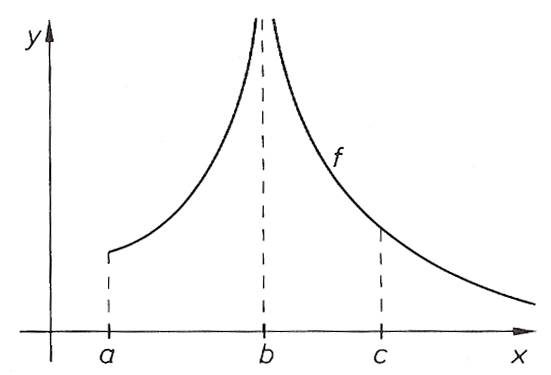
\includegraphics[width=4.5cm]{./bilder/unbeschraenkteFunktion.png}\\
    unbeschr\"ankte Funktion
  \end{multicols}
  
  
    
    
\subsubsection{Prinzip der Restfl\"ache}
  Wenn $\lim\limits_{t \rightarrow \infty} \int\limits^{\infty}_{t} f(x) dx = 0$, dann konvergiert
  $\int\limits_a^{\infty} f(x) dx$ und umgekehrt.

\subsubsection{Majorantenprinzip (konvergent)}
  Um nachzuweisen, ob eine Funktion $|f(x)| \geq 0$ konvergiert, wird eine zweite
  Funktion $g(x) \geq |f(x)|$ (Majorante) gesucht. Konvergiert $\int\limits_a^{\infty} g(x) dx$,
  dann konvergiert auch $\int\limits_a^{\infty} f(x) dx$. ($x \in [a, \infty)$)

\subsubsection{Minorantenprinzip (divergent)}
  Um nachzuweisen, ob eine Funktion $f(x)$ divergiert, wird eine zweite
  Funktion $0 \leq g(x) \leq f(x)$ (Minorante) gesucht. Divergiert
  $\int\limits_a^{\infty} g(x) dx$,
  dann divergiert auch $\int\limits_a^{\infty} f(x) dx$. ($x \in [a, \infty)$)
  
\section{Funktionsgraphen}
\begin{tabular}{lll}
\parbox{5.5cm}{
  \textbf{e-Funktion} \\
  %%$$e^x=\lim_{n \to \infty} (1+\frac{x}{n})^n$$       
  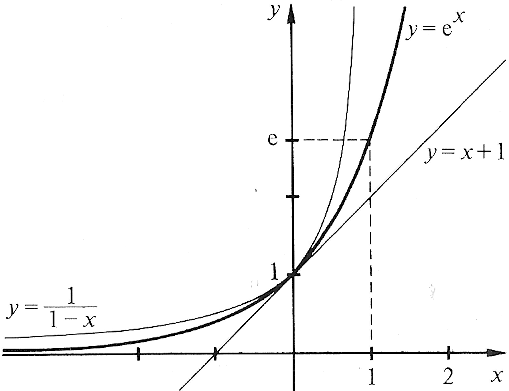
\includegraphics[width=4.5cm]{./bilder/funktionen_e.png} \\ \\
  
  \textbf{Logarithmus-Funktion}\\
  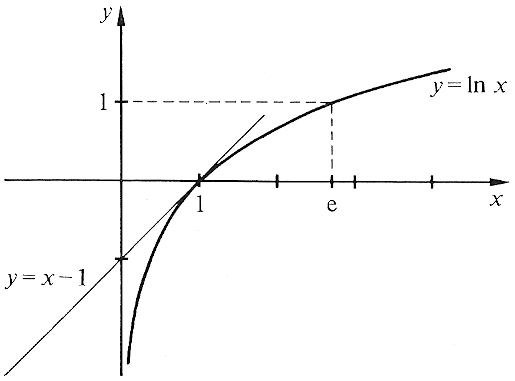
\includegraphics[width=4.5cm]{./bilder/funktionen_ln.png} 
}
& \parbox{5.5cm}{
  \textbf{Trigonometrische Funktionen}\\
  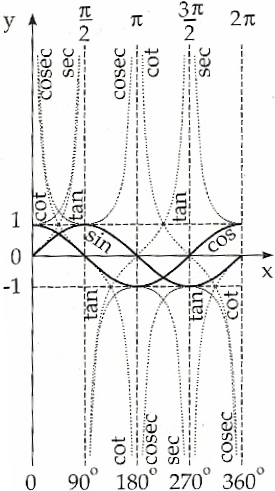
\includegraphics[width=4.5cm]{./bilder/funktionen_trigo.png} 
}
& \parbox{7cm}{
  \textbf{Hyperbel Funktionen}\\
  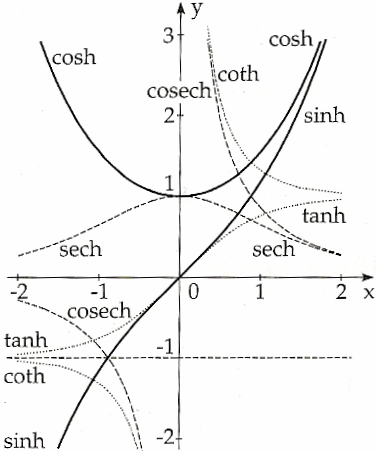
\includegraphics[width=6cm]{./bilder/funktionen_hyperbel.png} 
}
\end{tabular}

\section{Anwendung der Differential- und Integralrechnung}

\subsection{Beschreibungungsvarianten}
  \begin{minipage}[t]{3.5cm}
    Funktion (explizit) \\
    $ y = f(x)$ \\
        \tiny{(Bronstein Form 3.425)}
  \end{minipage}
  \begin{minipage}[t]{6cm}    
    Koordinatengleichung (implizit) \\
    $ F(x,y) = 0 $ \\
        \tiny{(Bronstein Form 3.424)}
  \end{minipage}
  \begin{minipage}[t]{5.5cm}    
    Parameterform \\
    $ \left( \begin{array} {l} x(t) \\ y(t) \end{array} \right) =
          \left( \begin{array} {l} \Psi(t) \\ \varphi(t) \end{array} \right)$\\
        \tiny{(Bronstein Form 3.426)}
  \end{minipage} 
  \begin{minipage}[t]{3cm}
      Polarform x\\
      $ r=f(\varphi) $ \\
        \tiny{(Bronstein Form 3.427)}
    \end{minipage}\\

  \textit{Hat man die explizite Form gegeben, so hat man automatisch die
  Implizite- und Parameter-Form}

\subsection{Umrechnen diverser Systeme \formelbuch{(197)}}
\begin{tabular}{lll}
Parameter 
  & $\Rightarrow$ explizit
  %& $x = f(t) \; \; y = g(t)$
  & $\Longrightarrow t = f(x);\; y = g(f(x))$\\
Ex- bzw. implizit 
  & $\Rightarrow$ Polar
  %& $y = f_1(x)$ bzw. $f_2(x,y) = C$
  & $\Longrightarrow$ Ersetze $x$ durch $r
\cos(\varphi)$ \& $y$ durch $r \sin(\varphi)$\\ 
Polar 
  & $\Rightarrow$ implizit
  %& $r = f(\varphi)$
  & $\Longrightarrow$ Ersetze $r \sin(\varphi)$ durch $y$, $r \cos(\varphi$ durch
  $x$, $r$ durch $\sqrt{x^2 + y^2}$\\ 
Polar
  & $\Rightarrow$ Parameterform
  %& $r = f(\varphi)$
  & $\Longrightarrow \left( \begin{array} {l} x(\varphi) \\ y(\varphi) \end{array} \right) =
          \left( \begin{array} {l} r(\varphi) \cos(\varphi) \\ r(\varphi) \sin(\varphi) \end{array}
          \right)$ \\
Explizit
  & $\Rightarrow$ Parameter
  %& $y = f(x)$
  & $\Longrightarrow \left( \begin{array} {l} x(t) \\ y(t) \end{array} \right) =
          \left( \begin{array} {l} x(t)) \\ t \end{array}
          \right)$ \\
Einzelner Punkt  
  & $\Rightarrow$ Polar
  %& $(x,\; y)$
  & $\Longrightarrow r = \sqrt{x^2 + y^2};\;
  \varphi = \begin{cases}\arctan(\frac{y}{x}) + \pi   &x < 0\\
             \arctan(\frac{y}{x})   & x > 0\\
             \frac{\pi}{2}      & x = 0;\; y > 0\\
             -\frac{\pi}{2}     & x = 0;\; y < 0\\
             \text{unbestimmt}    & x = y = 0\end{cases}$\\
\end{tabular}

\subsection{Kurvenarten\formelbuch{203ff}}
\begin{tabular}{llll}
\parbox{2.7cm}{
\textbf{ } \\
Implizit:\\
Bemerkung:\\
Polarform:\\
Parameterform:
}

\parbox{6cm}{
\textbf{Kreis\formelbuch{203}}\\
$(x-x_0)^2 + (y - y_0)^2 = r^2$\\
Mittelpunkt $(x_0, y_0)$; Radius $r$\\
$r = \frac{p}{1 + \epsilon \cos(\varphi)}; \epsilon = 0$ \\
$x=x_0 + R\cos(t), y=y_0 + R\sin(t)$
}

\parbox{8cm}{
\textbf{Ellipse\formelbuch{204}}\\
$(\frac{x-x_0}{a})^2 + (\frac{y-y_0}{b})^2 = 1$\\
Mittelpunkt $(x_0, y_0)$; Halbachsen $a$, $b$\\
$r = \frac{p}{1 + \epsilon \cos(\varphi)}; 0 < \epsilon < 1$\\
$x = a\cos(t), y = b\sin(t)$
}\\ \\

\parbox{2.7cm}{
\textbf {}\\
Implizit:\\
Bemerkung:\\
Polarform:\\
Parameterhform:
}

\parbox{6cm}{
\textbf{Hyperbel\formelbuch{206}}\\ 
$(\frac{x}{a})^2 - (\frac{y}{b})^2 = 1; -(\frac{x}{a})^2 + (\frac{y}{b})^2 =1$\\ 
\\
$r = \frac{p}{1 + \epsilon \cos(\varphi)}; \epsilon > 1$\\
$x= a \cosh(t), y = b \sinh(t) $
}

\parbox{8cm}{
\textbf{Parabel\formelbuch{209}}\\
$y= ax^2 + bx + c$\\
Parabeln mit Scheitelpunkt auf der vertikaler Achse\\
$r = \frac{p}{1 + \epsilon \cos(\varphi)}; \epsilon = 1$\\
$x=t, y = a t^2 + b t + c$
}\\ \\

\parbox{2.7cm}{
\textbf{} \\
Polarform:
}

\parbox{5cm}{
\textbf{Kardioide/Herzk. \formelbuch{99}} \\
$r = a(1+\cos(\varphi))$
}

\parbox{5cm}{
\textbf{Lemniskate ``$\infty$'' \formelbuch{101}} \\
$r = a\sqrt{2\cos(2\varphi)}$ 
}

\parbox{5cm}{
\textbf{Strophoide/harm. K. \formelbuch{96}} \\
$ r = -a \frac{\cos(2\varphi)}{\cos(\varphi)},(a>0) $ 
}

\end{tabular}

\subsection{Gleichungen\formelbuch{248}, Mittelwerte\formelbuch{19ff}}
\begin{tabular}{llll}
  \textbf{Tangentengleichung} &
  \textbf{Normalengleichung} &
  \textbf{Linearer Mittelwert} &
  \textbf{Quadratischer Mittelwert}\\
  $y-y_0=f'(x_0)(x-x_0)$ &
  $y-y_0=-\frac{1}{f'(x_0)}(x-x_0)$ &
  $\bar{f} = \frac{1}{b-a} \int\limits_{a}^{b} f(x)dx$ &
  $\bar{f} = \sqrt{\frac{1}{b-a} \int\limits_{a}^{b} f(x)^2dx}$
\end{tabular}
  
\subsection{Tangenten- \& Normalenabschnitt, Subtangente \&
Subnormale\formelbuch{249ff}}

\subsection{Abstandsformeln}
\begin{minipage}{6.5cm}
    \textbf{Hessesche Normalform\formelbuch{200f, 222}}\\
    $x\cdot \cos\varphi_0 +y\cdot \sin\varphi_0=r_0$\\
    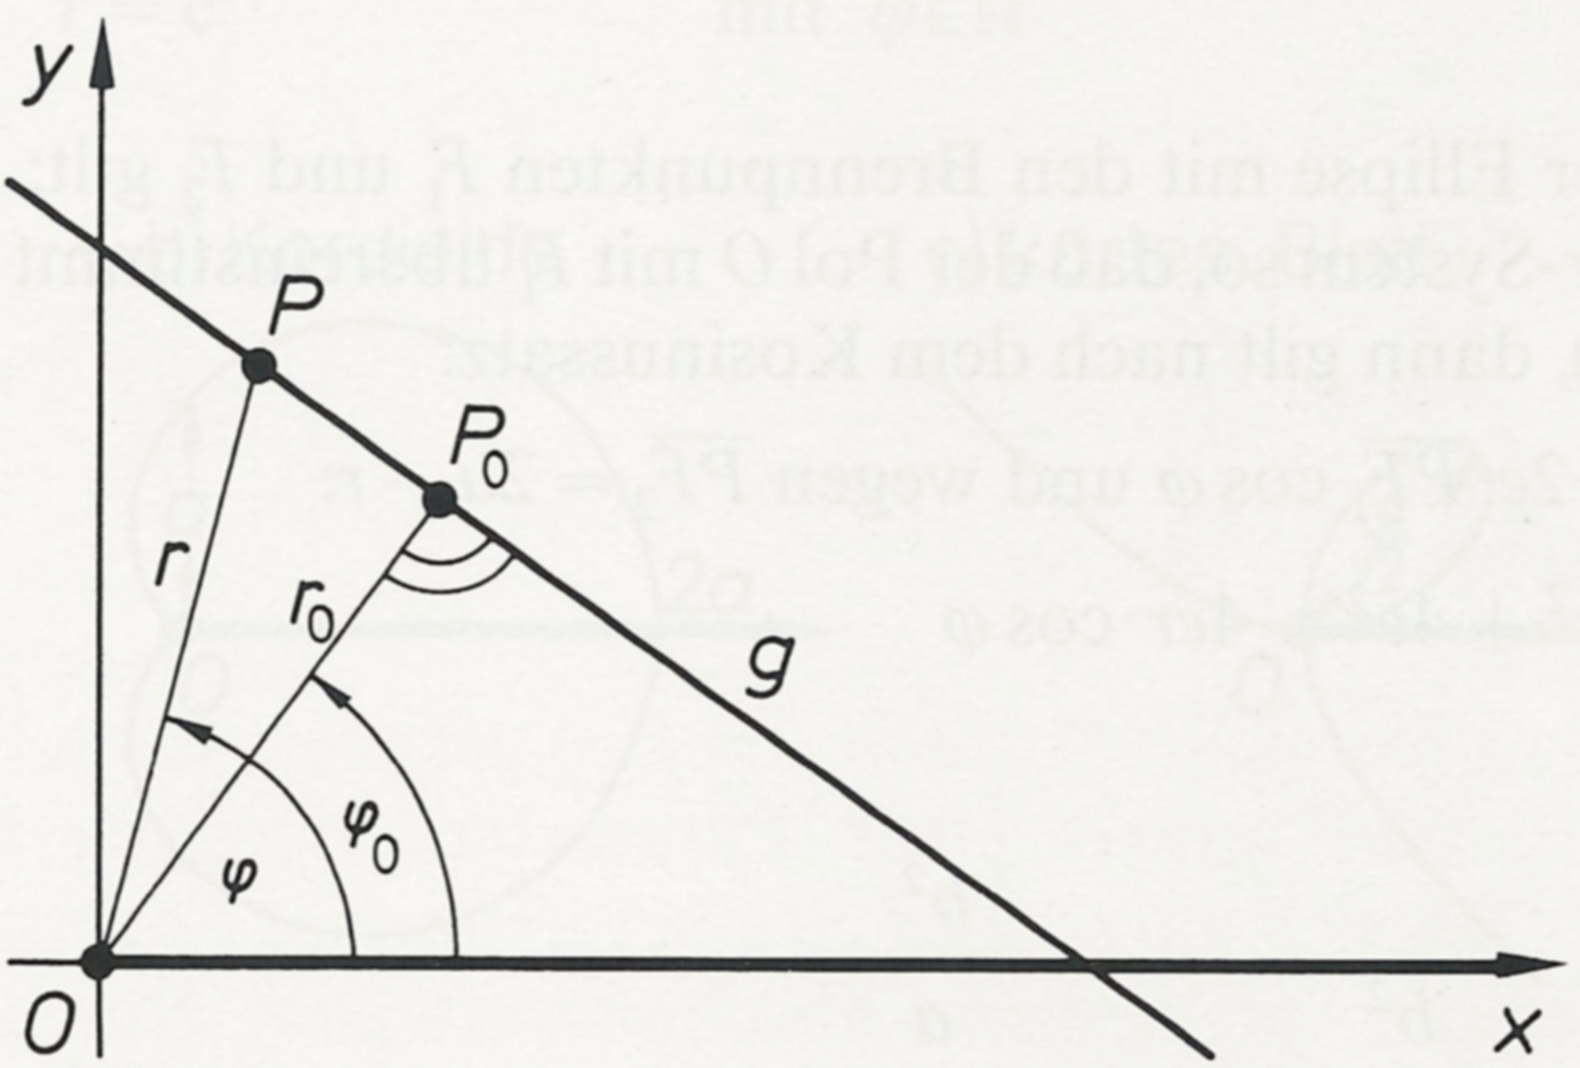
\includegraphics[width=2.8cm]{./bilder/hessenorm.png}
\end{minipage}
\begin{minipage}{6.5cm}
  \textbf{Geradengleichung} \\
  $y - y_0 = m (x - x_0)$
\end{minipage}
\begin{minipage}{6cm}
  \textbf{Abstand zum Ursprung} \\
  $\frac{|y_0 - m \cdot x_0|}{\sqrt{m^2 + 1}}$
\end{minipage}

\subsection{Berührung höherer Ordnung}
Zwei explizit gegebene Kurven $y = f(x)$ und $y = g(x)$ berühren einander im
Punkt P $x_0, y_0$ von der Ordnung $n$, wenn die Funktionswerte und die ersten
$n$ Ableitungen existieren und übereinstimmen.\\
$f(x_0) = g(x_0);\; f'(x_0) = g'(x_0);\; f''(x_0) = g''(x_0);\;\ldots ;
\;f^{(n)}(x_0) = g^{(n)}(x_0)\; \qquad f^{(n+1)}(x_0) \neq g^{(n+1)}(x_0)$

\subsection{Scheitel \formelbuch{254}}
Scheitelpunkte sind Extremalwerte der Krümmungs- bzw. Krümmungsradiusfunktion.
Falls bei $\kappa'(x)$ an der Stelle $x_0$ ein Vorzeichenwechsel besteht, existiert dort
eine Extremalstelle. 

\subsection{Wichtige Formeln\formelbuch{FF S60}}
\begin{tabular}{|p{4cm}|l|l|l|}
 \hline
 Geometrischer Begriff& karthesische Koordianten & Parameter Darstellung &
 Polarkoordinaten\\
 \hline
 Anstieg in $P_0$ $\in$ C & $f'(x_0)$ & $\frac{\dot \psi(t_0)}{\dot
 \varphi(t_0)}$ & $\frac{f'(\varphi_0)\sin \varphi_0 + f(\varphi_0)\cos
 \varphi_0}{f'(\varphi_0)\cos \varphi_0 - f(\varphi_0)\sin \varphi_0}$\\
 \hline
 Bogenl\"ange zwischen $P_1$,$P_2$ $\in$ C & $\int \limits{_a}^b
 \sqrt{1+(f'(x))^2}dx$ & $\int\limits_{t_2}^{t_2} \sqrt{\dot \varphi^2 + \dot\psi^2(t)}dt$ & 
 $\int\limits_{\varphi_1}^{\varphi_2}\sqrt{(f'(\varphi))^2+(f(\varphi))^2}d\varphi$\\
 \hline
 Kr\"umung in $P_0$ $\in$ C & $\frac{f''(x_0)}{(\sqrt{1+(f'(x_0))^2})^3}$ & 
  $\frac{\dot\varphi(t_0)\ddot
  \psi(t_0)-\dot\psi(t_0)\ddot\varphi(t_0)}{(\sqrt{\dot\varphi(t_0))^2+(\dot\psi(t_0))^2})`3}$&
  $\frac{2(f'(\varphi))^2-f(\varphi_0)f''(\varphi)+(f(\varphi_0))^2}{(\sqrt{(f'(\varphi_0))^2
  + (f(\varphi_0))^2})^3}$
  \\
 \hline 
 Fl\"acheninhalt einer Fl\"ache mit dem Rand C & $\int \limits_{b}^{a} f(x)dx)$ &
 $\frac{1}{2}\int\limits_{t_1}^{t_2}[\varphi(t)\dot\psi(t)-\dot\varphi(t)\psi(t)]dt$
 & $\frac{1}{2}\int\limits_{\varphi_1}^{\varphi_2}(f(\varphi))^2d\varphi$ \\
 \hline
 Volumen eines Rotationsk\"orpers mit dem Meridian C &
 $\pi\int\limits_{a}^{b}(f(x))^2dx$ &
 $\pi\left|\int\limits_{t_1}{t_2}(\psi(t))^2\dot\varphi(t)dt\right|$ &
 $\pi\left|\int\limits_{\varphi_1}^{\varphi_2}f^2(\varphi)\sin ^2
 \varphi[f'(\varphi)\cos \varphi - f(\varphi)\sin \varphi ]d \varphi \right|$
 \\
 \hline
 Oberl\"acheninhalt eines Rotationsk\"orpers mit dem Meridian C &
 $2\pi\int\limits_{a}^{b}\left|f(x)\right|\sqrt{(1+(f'(x))^2}dx$ &
 $2\pi\int\limits_{t_1}^{t_2}\left|\psi(t)\right|\sqrt{\dot\varphi^2(t)+\dot\psi^2(t)}dt$
 &
 $2\pi\int\limits_{\varphi_1}^{\varphi_2}\left|f(\varphi)\sin
 \varphi\right|\sqrt{(f'(\varphi))^2+(f(\varphi))^2}d\varphi$
 \\
 \hline
\end{tabular}

%  \renewcommand{\arraystretch}{2}
%  \begin{tabular}[c]{ | p{5.1cm} | p{5.4cm} | l | }
%    \hline
%   \textbf{Cartesisch} & \textbf{Parameter} & \textbf{Polar} \\
%    \hline
%    \multicolumn{3}{| l |}{\textbf{Anstieg einer Kurve, Ableitung, 2.
%    Ableitung}} \\
%      \hline   
%      $y'=f'(x_o) \quad y'' = f''(x_0)$ & 
%      $y'=\frac{\dot{y}}{\dot{x}} \quad 
%      y'' = \frac{\dot{x} \ddot{y} - \dot{y}\ddot{x}}{\dot{x}^3}$ &
%      $y'=\frac{r'(\varphi) \sin(\varphi) + r(\varphi) \cdot
%      \cos(\varphi)}{r'(\varphi) \cos(\varphi)-r(\varphi) \cdot \sin(\varphi)}$
%      \\
%    
%    \hline
%    \multicolumn{3}{| l |}{\textbf{Bogenlänge \formelbuch{233, 466}}} \\
%      \hline
%      $s=\int\limits_a^b{\sqrt{1+(f'(x))^2}dx}$ & 
%      $|s|=\int\limits_{t_1}^{t_2}{\sqrt{\dot{x}^2(t)+\dot{y}^2(t)}dt}$ &  
%       
%   	$|s|=\int\limits_{\varphi_1}^{\varphi_2}{\sqrt{(r'(\varphi))^2+((\varphi))^2}d\varphi}$\\
%   
%   \hline    
%   \multicolumn{3}{| l |}{\textbf{Krümmung ebener Kurven \formelbuch{236}}}\\
%     \hline
%     $\kappa=\frac{f''(x)}{(\sqrt{1+(f'(x))^2})^3}$ &
%     $\kappa=\frac{\dot{x}(t)\ddot{y}(t)-\dot{y}(t)\ddot{x}(t)}{(\sqrt{(\dot{x}(t))^2+(\dot{y}(t))^2})^3}$ &
%   $\kappa=\frac{2(r'(\varphi))^2-r(\varphi)r''(\varphi)+(r(\varphi))^2}{(\sqrt{(r'(\varphi))^2+(r(\varphi))^2})^3}$\\     
%   
%   \hline
%   \multicolumn{3}{| l |}{Konvex (Linkskurve): $\kappa \geq 0 \qquad$ Streng
%   konvex: $\kappa > 0 \qquad$ Wendepunkt: $\kappa = 0 \qquad$ Analog für konkav}\\
%   
%   \hline
%   \multicolumn{3}{| l |}{\textbf{Krümmungskreisradius \formelbuch{236f}}} \\
%   \hline
%   $r = \left|\frac{(\sqrt{1+(f'(x))^2})^3}{f''(x)} \right|$ &
%   $r = \left|\frac{(\sqrt{(\dot{x}(t))^2+(\dot{y}(t))^2})^3}
%   {\dot{x}(t)\ddot{y}(t)-\dot{y}(t)\ddot{x}(t)} \right|$ & 
%   $r = \left|\frac{(\sqrt{(r'(\varphi))^2+(r(\varphi))^2})^3}
%   {2(r'(\varphi))^2-r(\varphi)r''(\varphi)+(r(\varphi))^2} \right|$ \\
%   
%   \hline    
%   \multicolumn{3}{| l |}{\textbf{Flächeninhalt \formelbuch{465}}} \\
%     \hline
%     $A=\int\limits_a^b{f(x)}dx$  & 
%     $A=\frac{1}{2}\int\limits_{t_1}^{t_2}{[x(t)\dot{y}(t)-\dot{x}(t)y(t)]dt}$ &
%   $A=\frac{1}{2}\int\limits_{\varphi_1}^{\varphi_2}{(r(\varphi))^2d\varphi}$\\  
%     
%  \hline    
%  \multicolumn{3}{| l |}{\textbf{Volumen \formelbuch{467}}} \\
%    \hline
%    $V=\pi\int\limits_a^b(f(x))^2dx$ & 
%      $V=\pi\left|\int\limits_{t_1}^{t_2}{(y(t))^2\dot{x}(t)dt}\right|$ &   
%    $V=\pi\left|\int\limits_{\varphi_1}^{\varphi_2}{r^2(\varphi)\sin^2\varphi[r'(\varphi)\cos(\varphi)-r(\varphi)\sin(\varphi)]d\varphi}\right|$\\
%      
%    \hline    
%    \multicolumn{3}{| l |}{\textbf{Oberflächeninhalt \formelbuch{466f}}} \\
%      \hline
%      $O=2\pi\int\limits_a^b{|f(x)|\sqrt{1+(f'(x))^2}dx}$ &  
%     
%   $O=2\pi\int\limits_{t_1}^{t_2}{|y(t)|\sqrt{\dot{x}^2(t)+(\dot{y}^2(t))}dt}$ & $O=2\pi\int\limits_{\varphi_1}^{\varphi_2}{|r(\varphi)\sin\varphi|\sqrt{(r'(\varphi))^2+(r(\varphi))^2}d\varphi}$\\
%      \hline
%  \end{tabular}
%  \renewcommand{\arraystretch}{1}
\subsection{Orthogonaltrajektorien}
\begin{tabular}{ll}
\parbox{4.5cm}{
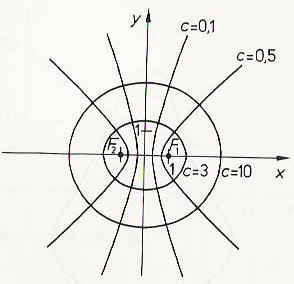
\includegraphics[height=4cm]{./bilder/orthoTrajekt.png}
}
& \parbox{14.5cm}{
Die orthogonalen Trajektorien schneiden alle Kurven der gegebenen Kurvenschar
$y=f(x,c)$ im rechten Winkel.\\
Die DGL $F(x,y,y')$ der Kurve bestimmen, anschliessend $y'$ durch
$-\frac{1}{y'}$ ersetzen.\\
$\Rightarrow$ ergibt die DGL der orthogonalen Trajektorien.\\
 \\
Die Kreise sind Orthogonaltrajektorien der Hyperbeln und umgekehrt.
}
\end{tabular}

\section{Reihen\formelbuch{460, 465, 1066}}

\subsection{Zahlenreihen\formelbuch{460}}
  $ s_n = \sum\limits_{k=1}^{n} a_k \qquad $ ist eine (unendliche) Reihe. Sie
  ist die Folge von Partialsummen einer bestehenden Folge $a_n$.

\subsubsection{Konvergenz, Divergenz\formelbuch{460}}
Konvergiert die Reihe $\langle s_n \rangle$ gegen die Summe $ s =
\sum\limits_{k=1}^{\infty} a_k $ so ist sie konvergent. Existiert der GW nicht, so ist sie divergent.

\subsubsection{Geometrische Reihe}
Es sei $a_1\in\mathbb R$ und $q\in\mathbb R \backslash \{0;1\}$, dann erh"alt
man aus der geometrischen Folge $\langle a_k \rangle$ mit $a_k=a_1 \cdot
q^{k-1}$ die geometrische Reihe $\langle s_n \rangle$ mit
\textbf{$s_n= \sum\limits_{k=1}^{n} a_1 \cdot q^{k-1}=a_1 \cdot
\frac{1-q^n}{1-q}$\\}
\paragraph{Monotonie}
\begin{tabular}{ll}
$s_n \leq 0$&$\to$ (streng) monoton Fallend\\
$s_m \geq 0$&$\to$ (streng) monoton Steigend\\
$0 < q \leq 1$&$\to$ (streng) monoton Fallend\\
$0 < q \geq 1$&$\to$ (streng) monoton Stieigend\\
\end{tabular}

\subsubsection{Harmonische Reihe}
Aus der Folge $\langle a_k \rangle$ mit $a_k=\frac{1}{k}$ erhalten wir die
harmonisch Reihe mit $\langle s_n \rangle$ mit
\textbf{$s_n=\sum\limits_{k=1}^{n}
\frac{1}{k}=1+\frac{1}{2}+\frac{1}{3}+\dotsc+\frac{1}{n}$}
\subsubsection{Konvergenzkriterien}

\paragraph{Cauchy-Kriterium} 
  Wenn zu jedem $\varepsilon > 0$ ein Index $n_0$ existiert, so dass f"ur alle
  $m > n > n_0$ gilt: \\ $\left| \sum\limits_{k=n}^m a_k \right| < \varepsilon$, dann konvergiert die Reihe, ansonsten divergiert sie.

\paragraph{lim = 0\formelbuch{461}}
  Wenn die Reihe $ \sum\limits_{n=1}^{\infty} a_n $ konvergent ist, so ist
  $\lim\limits_{n \to \infty} a_n = 0$. \hspace{2cm} Aber NICHT UMGEKEHRT!

\paragraph{Divergenz}
  Ist $<a_n>$ divergent oder ist $\lim\limits_{n \to \infty} a_n \neq 0$, so
  ist die Reihe $ \sum\limits_{n=1}^{\infty} a_n $ divergent.

\paragraph{Majorantenkriterium\formelbuch{469}}
  Ist die Reihe $ \sum\limits_{n=1}^{\infty} c_n $ konvergent, so konvergiert
  auch die Reihe $ \sum\limits_{n=1}^{\infty} a_n $ f"ur $|a_n| \leq c_n$ (absolut). \\ Dies gilt auch f"ur $|a_n| \leq c_n$ erst ab einer Stelle $n_0 \in \mathbb{N}$.

\paragraph{Minorantenkriterium}
  Ist die Reihe $ \sum\limits_{n=1}^{\infty} d_n $ gegen $+\infty$ divergent, so
  gilt dies auch f"ur die Reihe $ \sum\limits_{n=1}^{\infty} a_n $ bei $a_n \geq d_n$. \\ Dies gilt auch f"ur $a_n \geq d_n$ erst ab einer Stelle $n_0 \in \mathbb{N}$.

\paragraph{Reziprokkriterium}
  $ s = \sum\limits_{n=1}^{\infty} \frac{1}{n^\alpha} $ ist konvergent f"ur
  $\alpha > 1$ und divergent f"ur $\alpha \leq 1$.

\paragraph{Quotientenkriterium\formelbuch{464}}
  $ \lim\limits_{n \to \infty} \left|\frac{a_{n+1}}{a_n}\right| = \alpha $ der
Reihe $ \sum\limits_{n=1}^{\infty} a_n $ \\ $\alpha < 1 \Rightarrow$ (absolut) konvergent \hspace{3cm}
  $\alpha > 1 \Rightarrow$ divergent \hspace{4cm} 
  $\alpha = 1 \Rightarrow$ keine Aussage!

\paragraph{Wurzelkriterium\formelbuch{464f}}
  $ \lim\limits_{n \to \infty} \sqrt[n]{\left|a_n\right|} = \alpha $ der Reihe $
\sum\limits_{n=1}^{\infty} a_n $ \\ $\alpha < 1 \Rightarrow$ (absolut) konvergent\hspace{3cm}
  $\alpha > 1 \Rightarrow$ divergent \hspace{4cm} 
  $\alpha = 1 \Rightarrow$ keine Aussage!

\paragraph{Integralkriterium\formelbuch{465}}
  $ \sum\limits_{n=1}^{\infty} f(n) $ ist konvergent, wenn das uneigentliche
Integral $ \int\limits_{1}^{\infty} f(x) dx $ konvergent ist. \\ Gilt nur, wenn $f$ auf $ [1, \infty) $ definiert und monoton fallend ist. Zudem muss $ f(x) \geq 0 $ f"ur alle $x \in [1, \infty)$ sein.
 
\paragraph{Leibniz-Kriterium\formelbuch{466}}
  Die \textbf{alternierende} Reihe $ \sum\limits_{n=1}^{\infty} a_n $ ist
  konvergent, wenn die Folge $<\left|a_n\right|>$ eine monoton fallende Nullfolge ($\lim\limits_{n \to \infty} \left|a_n\right| = 0 $) ist. \\ 
  Monotonie mittels Verh"altnis ($ \left|\frac{a_{n+1}}{a_n}\right| $),
  Differenz ($ |a_{n+1}| - |a_n| $) oder \textit{vollst"andiger Induktion} beweisen.\\

\paragraph{Absch"atzung Restglied einer alternierenden konvergenten
  Reihe\formelbuch{466,470}}\qquad $|R_n| = |s-s_n|\leq |a_{n+1}|$


\subsubsection{Bedingte und Absolute Konvergenz\formelbuch{465}}
  Eine Reihe $\sum\limits_{n=1}^{\infty}a_n$ heisst \textbf{absolut konvergent},
wenn die Reihe $\sum\limits_{n=1}^{\infty}|a_n|$ konvergent ist.\\
\textbf{Bedingt Konvergent:} Eine Reihe hat durch Umordnen einen anderen
Grenzwert oder wird divergent.\\
\textbf{Unbedingt Konvergent:} Durch Umordnen \"andert sich der Grenzwert nicht.

\subsubsection{Produkt von absolut konvergenten Reihen\formelbuch{466}} 
  Gegeben sei: $\sum a_n=a$, \quad $\sum b_n=b, \quad \sum c_n = (\sum a_n)
\cdot (\sum b_n) = c \quad $ so ist $ \quad c_n=\sum a_kb_{n-k+1} \quad $ und $ \quad c = a \cdot b $



\subsection{Potenzreihen}

\paragraph{Definition\formelbuch{432}} 

  Die Reihe $ \sum\limits_{n=0}^{\infty} a_n (x-x_0)^n $ heisst Potenzreihe mit
Entwicklungspunkt $x_0$ und Koeffizienten $a_n$.

\begin{tabular}{l l l}
\textbf{Geometrische Reihe\formelbuch{19}}
  & $ \frac{a}{1-x} = a \cdot \sum\limits_{n=0}^{\infty} x^n$
  & $(|x| < 1) \qquad$ Beidseitiges $\int \quad\Rightarrow\quad -a \cdot \ln{|x-1|} 
= a \cdot \sum\limits_{n=1}^{\infty} \frac{x^{n}}{n} $ \\
\textbf{Binominalreihe} 
  & $ (1+x)^\alpha = \sum\limits_{n=0}^\infty \binom{\alpha}{n} x^n$
  & $x \in (-1,1)$ \\
\textbf{Taylor-Reihe\formelbuch{474}}
  & $ \sum\limits_{n=0}^{\infty} \frac{f^{(n)}(x_0)}{n!}\cdot(x-x_0)^n$
  & Taylor-Reihe von f bez"uglich der Stelle $x_0$ \\
\textbf{E-Funktion}
  & \multicolumn{2}{l}{$e = \lim\limits_{n\to\infty} \left(1+\frac{1}{n}\right)^n = 
  \sum\limits_{k=0}^{\infty}{\frac{1}{k!}} = 1 + \frac{1}{1} + \frac{1}{1\cdot 2} +
  \frac{1}{1\cdot 2\cdot 3}  + \frac{1}{1\cdot 2\cdot 3\cdot4} + \cdots$}
\end{tabular}

\subsubsection{Konvergenz\formelbuch{472}}
  Gegeben sei die Potenzreihe $ \sum\limits_{n=0}^{\infty} a_n x^n $ mit $
\lim\limits_{n \to \infty} \sqrt[n]{|a_n|} = a $ \\ F"ur $ a=0 $ ist die Potenzreihe f"ur alle $ x \in \mathbb{R} $ absolut
konvergent. \\ F"ur $ a>0 $ ist die Potenzreihe f"ur alle $x$ mit 
  $ \left\{   
    \begin{array}{l} 
      |x| < \frac{1}{a} = \rho \Rightarrow \text{ absolut konvergent.} \\
      |x| > \frac{1}{a} = \rho \Rightarrow \text{ divergent.}
    \end{array} 
  \right. $ \\
  Ist die Folge $<\sqrt[n]{|a_n|}>$ nicht beschr"ankt, so ist die Potenzreihe
nur f"ur $x=0$ konvergent.

\subsubsection{Konvergenzradius\formelbuch{472}}
  Jeder Potenzreihe kann ein Konvergenzradius $\rho$ zugeordnet werden. Wobei
gilt $\rho = \frac{1}{a}$ mit $a = \lim\limits_{n \to \infty} \sqrt[n]{|a_n|} $.
\\ F"ur $a = 0$ gilt $\rho = \infty$. Wenn a nicht exisitiert (Folge divergent) ist $\rho = 0$. \\ Berechnung mittels Quotientenkriterium: $ \rho = \lim\limits_{n \to \infty} \left| \frac{a_n}{a_{n+1}} \right|$

\subsubsection{Differentiation}
  Alle Potenzreihen mit einem $\rho > 0$ sind f"ur alle $x \in (-\rho, \rho)$
beliebig oft (gliedweise) differenzierbar. \\ Der Potenzradius $\rho$ ist bei allen Ableitungen gleich demjenigen der Ursprungsfunktion. $\rho_{f} = \rho_{f^{(i)}}$.
$$ f(x) = \sum\limits_{n=0}^{\infty} a_n x^n  \qquad 
   f'(x) = \sum\limits_{n=1}^{\infty} n \cdot a_n x^{n-1 } \qquad 
   f''(x) = \sum\limits_{n=2}^{\infty} n(n-1) \cdot a_n x^{n-2} \qquad 
   f^{(i)}(x) = \sum\limits_{n=i}^{\infty} n(n-1)\cdot \ldots \cdot (n-i+1)\cdot a_n x^{n-i} $$ 
  \textbf{Bemerkung:} Startwert ($n=0$) nur erh"ohen, wenn bei $x^n, n$ negativ
werden w"urde!

\subsubsection{Integration}
 \paragraph{Unbestimmtes Integral}
$\int \sum\limits_{n=0}^{\infty} a_n x^n dx = 
\sum\limits_{n=0}^{\infty} a_n \int x^n dx = 
\sum\limits_{n=0}^{\infty} \frac{a_n}{n+1}\cdot x^{n+1} \qquad \text{ für alle } x \in (-\rho, \rho).$
\paragraph{Bestimmtes Integral}
$\int\limits_0^x \sum\limits_{n=0}^{\infty} a_n t^n dt = 
\sum\limits_{n=0}^{\infty} \frac{a_n}{n+1}\cdot x^{n+1} \qquad \text{ für alle } x \in (-\rho, \rho).$

\section{Differentialgleichungen \formelbuch{543}}

\subsection{L"osen von Differentialgleichungen}

\subsubsection{Trennung von Variabeln \formelbuch{545}}
\begin{tabular}{p{4cm}p{1.5cm}p{10.5cm}}
\textbf{Form:} $y' = f(x) g(y)$ &
\textbf{Vorgehen:}              &
$\frac{y'}{g(y)} = f(x)$, nun ist die DGL beidseitig nach x integrierbar\\  &&
($dx = \frac{dy}{y'}$): $\int \frac{1}{g(y)} dy = \int f(x) dx$ 
\end{tabular}

\subsubsection{Lineartermsubstitution \formelbuch{545}}
\begin{tabular}{p{4cm}p{1.5cm}p{10.5cm}}
\textbf{Form:} $y'=f(ax+by+c)$   &
\textbf{Vorgehen:}               &
1. Substitution: $z=ax+by+c \qquad z'=a+by' =a+bf(z)$\\ &&
$\int\frac{z'}{a+bf(z)} = \int 1$
\end{tabular}

\subsubsection{Gleichgradigkeit}
\begin{tabular}{p{4cm}p{1.5cm}p{10.5cm}}
\textbf{Form:} $y'=f(\frac{y}{x})$ &
\textbf{Vorgehen:}                &
1. Substitution: $z=\frac{y}{x} \qquad
z'=\frac{1}{x}(f(z)-z)$
\end{tabular}

\subsubsection{Lineare Differentialgleichungen 1. Ordnung \formelbuch{546}}
\begin{tabular}{p{4cm}p{1.5cm}p{10.5cm}}
\textbf{Form:} $ y'+f(x)y = g(x) $ &
\textbf{Vorgehen:}                 &
$ y=e^{-\int f(x) dx}(k+\int g(x)e^{\int f(x)dx}dx)$
\end{tabular}

\subsection{Lineare Differentialgleichung 2. Ordnung mit konstanten 
Koeffizienten \formelbuch{564}}
\begin{tabular}{p{8cm}p{8cm}}
\textbf{Form:} $y''+a_1\cdot y'+a_0\cdot y=f(x)$  &
\textbf{St"orglied:} $f(x)$\\
\textbf{Homogene Differentialgleichung:} $f(x)=0$ &
\textbf{Inhomogene Differentialgleichung:} $f(x)\neq 0$
\end{tabular}

\subsubsection{Allgemeine L"osung einer homogenen DGL:\quad\subsubadd{$\quad
Y_H$}}
\textbf{Charakteristisches Polynom}
$\qquad\underline{\lambda^2+a_1\cdot\lambda+a_0=0}$ \hspace{1cm}von
$\qquad\underline{y''+a_1\cdot y'+a_0\cdot y=0}$ 
$\qquad(\lambda_{1,2} = -\frac{a_1}{2} \pm \frac{\sqrt{a_1^2 - 4a_0}}{2})$\\ \\
\begin{tabular}{p{8cm}p{8cm}}
Falls $\lambda_1\neq \lambda_2$ und $\lambda_{1,2} \in R$:&
$Y_H=A_1e^{\lambda_1x}+A_2e^{\lambda_2x}$\\
Falls $\lambda_1=\lambda_2$ und $\lambda_{1,2} \in R$:    &
$Y_H=e^{\lambda_1x}(A_1+A_2\cdot x)$\\
Falls $\lambda_{1,2}=-\frac{a_1}{2}\pm j\alpha$:          &
$Y_H=e^{-\frac{1}{2}a_1x}(A_1cos(\alpha x) +A_2sin(\alpha x))$\\
\end{tabular}

\subsubsection{Allgemeine L"osung einer inhomogenen
DGL:\quad\subsubadd{$y=Y_H+y_P$}}

\subsubsection{Grundl"oseverfahren einer inhomogenen DGL:\quad\subsubadd{$\quad
y_P$}} Homogene DGL: $y''+a_1\cdot y'+a_0\cdot y=0$  f"ur die  $g(x_0)=0$  und
$g'(x_0)=1$  gilt, ist:\\
$$y_P(x)=\int\limits_{x_o}^{x} g(x+x_0-t)\cdot f(t)dt$$\\
die partikul"are L"osung von $y''+a_1\cdot y'+a_0\cdot y=f(x)$

\subsubsection{Der Ansatz einer inh. DGL in Form des
St"orgliedes:\quad\subsubadd{$\quad y_P$}} $f(x)=p_n(x)$\hspace{9cm}($p_n(x)$
und $q_n(x)$ sind Polynome vom gleichen Grad)\\
\begin{tabular}{p{8cm}p{4cm}}
Fall a: $a_0\neq 0$:          & $y_P = q_n(x)$\\
Fall b: $a_0 = 0 , a_1\neq 0$:& $y_P=x\cdot a_n(x)$\\
Fall c: $a_0=a_1=0$:          & $y_P=x^2\cdot q_n(x)$\\
\end{tabular}\\
$f(x)=e^{bx}\cdot p_n(x)$\\
\begin{tabular}{p{8cm}p{4cm}}
Fall a: $b$ nicht Nullstelle des char. Polynoms:    &
$y_P=e^{bx}\cdot q_n(x)$\\
Fall b: $b$ einfache Nullstelle des char. Polynoms: &
$y_P=e^{bx}\cdot x \cdot q_n(x)$\\
Fall c: $b$ zweifache Nullstelle des char. Polynoms:&
$y_P=e^{bx}\cdot x^2\cdot q_n(x)$\\
\end{tabular}\\
$f(x)=y''+a_1y'+a_0y=e^{cx}(p_n(x)\cos{bx}+q_n(x)\sin{bx})$\\
\begin{tabular}{p{8cm}p{8cm}}
Fall a: $c+jb$ \textbf{nicht} L�sung der char. Gleichung &
$y_p=e^{cx}(r_n(x)\cos{bx}+s_n(x)\sin{bx})$ \\
Fall b: $c+jb$ L�sung der char. Gleichung &
$y_p=e^{cx}x(r_n(x)\cos{bx}+s_n(x)\sin{bx})$\\
\end{tabular}


\subsubsection{Superpositionsprinzip}
$f(x)=c_1f_1(x)+c_2f_2(x)$\\
\begin{tabular}{p{8cm}p{4cm}}
$y_1$ ist spezielle L"osung der DGL &
$y''+a_1\cdot y'+a_0\cdot y=c_1f_1(x)$ \\
$y_2$ ist spezielle L"osung der DGL &
$y''+a_1\cdot y'+a_0\cdot y=c_2f_2(x)$ \\
dann ist:                          &
$y_P=c_1y_1+c_2y_2$\\
\end{tabular}

\subsection{Lineare Differentialgleichung n. Ordnung mit konstanten 
Koeffizienten \formelbuch{554}}
\begin{tabular}{p{8cm}p{8cm}}
\textbf{Form:} &
$\sum\limits_{k=0}^na_ky^{(k)}= y^{(n)}+a_{n-1}\cdot y^{(n-1)}+\ldots +a_0\cdot y=f(x)$\\
\textbf{Algemeine L"osung der homogenen DGL:} &
$g=c_1g_1+c_2g_2+\ldots +c_kg_k$\\
\end{tabular}

\subsubsection{Homogene L"osungen}
\begin{tabular}{lll}
Fall a: r reelle L"osungen $\lambda_1$: 
  & $y_1=e^{\lambda_1x}$, $y_2=xe^{\lambda_1x}$, \ldots
  ,$y_r=x^{r-1}e^{\lambda_1x}$ 
  & Starke D"ampfung / Kriechfall\\
Fall b: $k$ komplexe L"osungen $\lambda_2=\alpha +j\beta$: 
  &$y_1=e^{\alpha x}\cos(\beta x)$, \ldots, $y_k=e^{\alpha x}x^{k-1}\cos(\beta
x)$
  & Schwache D"ampfung /\\
  &$y_{k+1}=e^{\alpha x}\sin(\beta x)$, \ldots, $y_{2k}=e^{\alpha
x}x^{k-1}\sin(\beta x)$
  & Schwingfall\\
\end{tabular}

\subsubsection{Allgemeinste L"osung des partikul"aren Teils:}
$$\underbrace{\sum_{k=0}^n a_k y^{(k)}}_{f(y,y',y'',\ldots)} = \underbrace{e^{\alpha x} (p_{m1}(x) \cos (\beta x) + q_{m2}(x) \sin (\beta x))}_{\text{St"orglied}}$$
Unterscheide die L"osungen des charakteristischen Polynoms
($\lambda$):\hspace{5.5cm}mit m = max(m1, m2)\\
\begin{tabular}{p{8cm}p{8.5cm}}
Fall a: $\alpha + j\beta \neq \lambda$, so ist &
$y_P = e^{\alpha x}(r_m(x)\cos(\beta x) + s_m(x) \sin(\beta x))$\\
Fall b: $\alpha + j\beta$  ist u-fache L"osung von $\lambda$, so ist &
$y_P = e^{\alpha x} x^u (r_m(x) \cos(\beta x) + s_m(x) \sin(\beta x))$\\
&
u-fache Resonanz

\end{tabular}

\subsubsection{Grundl"oseverfahren}
\begin{tabular}{p{12cm}p{5cm}}
$\begin{pmatrix}
g(x_0)=  & 0 & = & c_1g_1(x_0)+c_2g_2(x_0)+\ldots +c_n(x_0)\\
g'(x_0)= & 0 & = & c_1g_1'(x_0)+c_2g_2'(x_0)+\ldots +c_ng_n'(x_0)\\
\vdots  & \vdots & \\                            
g^{(n-1)}(x_0)= & 1 & = & c_1g_1^{(n-1)}(x_0)+c_2g_2^{(n-1)}(x_0)+\ldots
+c_ng_n^{(n-1)}(x_0)
\end{pmatrix}$ &
\begin{minipage}[t]{5cm}
ergibt $c_1,\ldots ,c_n$ f"ur\\
$y_{P}(x)=\int_{x_0}^x{g(x+x_0-t)f(t)dt}$
\end{minipage}
\end{tabular}

\subsubsection{Hornerschema\formelbuch{914}}
\begin{minipage}[t]{9cm}
- Pfeile $\Rightarrow$ Multiplikation\\
- Zahlen pro Spalte werden addiert\\
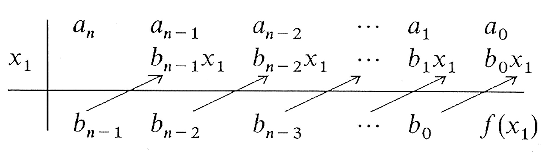
\includegraphics[width=6cm]{./bilder/Hornerschema_1.png}\\
$x_1 \Rightarrow$ Nullstelle (muss erraten werden!!)\\
oberste Zeile = zu zerlegendes Polynom
\end{minipage}
\begin{minipage}[t]{9cm}
\textbf{Beispiel:}\\
$f(x) = x^3-67x-126$\\
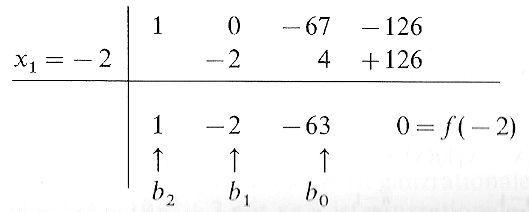
\includegraphics[width=6cm]{./bilder/Hornerschema_2.png}\\
$\Rightarrow f(x) = (x-x_1)(b_2x^2 + b_1x + b_0) = (x+2)(x^2-2x-63)$  
\end{minipage}

\subsection{Lineare Differentialgleichungssysteme erster Ordnung mit konstanten
Koeffizienten}
\begin{tabular}{p{8cm}p{8cm}}
\textbf{Form:}&
$\dot{x}=ax+by+f(t)$\\
&
$\dot{y}=cx+dy+g(t)$\\
\textbf{Die allgem. L"osung ergibt sich aus der DGL:}&
$\ddot{x}-(a+d)\dot{x}+(ad-bc)x=\dot{f}(t)-df(t)+bg(t)$\\
&
$y=\frac{1}{b}(\dot{x}-ax-f(t)))$\\
\end{tabular}

\subsection{D"ampfung}
\begin{itemize}
  \setlength{\itemsep}{1pt}
  \setlength{\parskip}{0pt}
  \setlength{\parsep}{0pt}
  
  \item Starke D�mpfung: $D>0$
  \item Grenzfall; $D=0$
  \item Schwingfall / schawache D"ampfung: $D<0$
\end{itemize}
Frequenz: $\omega = \frac{\sqrt{\left|D\right|}}{2}$
D�mpfung $\left|\delta\right| = \left|{\frac{a_1}{2}}\right|$
siehe: $\lambda_{1,2}= -\frac{a_1}{2}\pm \frac{\sqrt{{a_1}^2-4a_0}}{2}$


\end{document}